\chapter{Dynamic Semantics}
\label{sec:PolicyTrees}

\remark{
{\em Expected Outcome:} Reader understands how a temporal slice of Share Tree 
maps to a Policy Tree, and how they are compiled to OpenFlow tables. Reader 
appreciates the use and power of the conflict-resolution operators 
independently of the Share Tree.
Presentation of the Share Tree as a gatekeeper (or, the setting, the stage)
}

This chapter discusses the \sys compiler and runtime system that
implements share trees in a software-defined network.  Share trees,
discussed in the previous chapter, hold information about all
authorized requests: the type of request (\eg, access control,
bandwidth reservation, etc.), the flowgroup the request applies to,
the principal that made the request, and the start time and duration
of the request. All this information is needed for correct accounting
and to ensure that principals' privileges are not violated, but we can
use a much simpler data structure to configure the network.

\remark{In this paper, the conflict resolution idea has to be
  introduced with share trees!}  A \emph{policy tree} is a snapshot of
the share tree at a particular point in time that also strips away
information that is only needed for accounting. It only includes the
accepted requests and the conflict resolution operators.

The policy tree is a declarative data structure. To update the physical
network, it needs to be coupled with information from the
\emph{network information base} (NIB): the network topology, switches'
capabilities, and the locations of hosts.

\section{Policy Tree Semantics}
\label{sec:PolicyTree-Semantics}

We define the semantics of a Policy Tree as the
final action it produces on an individual packet, after it has
consolidated actions from all policies in the tree.\footnote{This
  semantic model, where the central controller conceptually sees all
  packets, is inspired by Frenetic~\cite{Foster:2010}.}
Because OpenFlow switches cannot directly implement these trees,
we linearize Policy Trees to \emph{network flow tables} (\Cref{sec:compilation}), which
\sys's runtime uses to configure switches (\Cref{sec:FullSystem}).
%{\color{red} We conclude with a theorem that this translation is correct.} % where did we put it?


\begin{figure}

\begin{displaymath}
\begin{array}{lrcl}
& H & = & \textrm{header names and ingress ports} \\
\textrm{patterns} & V & = & \textit{const} \mid \textit{prefix} \mid \star \\
\textrm{matches} & M & = & 
  \emptyset \mid \langle \overrightarrow{H,V} \rangle \\
\textrm{actions} & A & = & \textbf{Allow} \mid \textbf{Deny} 
  \mid \textbf{GMB}(n) \mid \textbf{0} \\
\textrm{conflict-resolution} & (+)  & = & A \rightarrow A \rightarrow A \\
\textrm{operators} \\
\textrm{policy atoms} & P & = & M \times A \\
\textrm{Policy Tree nodes} & D & = & (+_D) \times 2^P \\
\textrm{Policy Trees} & T & = & (+_P) \times (+_S) \times D \times 2^{T} \\
\textrm{packets} & K & = & \langle \overrightarrow{H,\mathit{const}} \rangle
\end{array}
\end{displaymath}

\fbox{$\mathit{cmb} : D \times K \rightarrow A$}
\begin{displaymath}
\begin{array}{l}
\mathit{cmb}((+,\{ \cdots (M_i,A_i) \cdots \}), K) = 
  A'_1 + \cdots + A'_k + \textbf{0} \\
\begin{array}{lrcl}
\textrm{where} & \{ A'_1, \cdots, A'_k \} & = & \{ A_i | M_i \cap K \ne \emptyset \}
\end{array}
\end{array}
\end{displaymath}

\fbox{$\mathit{eval} : T \times K \rightarrow A$}
\begin{displaymath}
\begin{array}{l}
\textit{eval}((+_P,+_S,D,\{ T_1,\cdots, T_n \}), K) = \textit{cmb}(D, K) +_P A_1 \\
\begin{array}{lrcl}
\textrm{where}
& A_1 & = & eval(T_1,K) +_S A_2 \\
& A_2 & = & eval(T_2,K) +_S A_3 \\
& \cdots \\
& A_n & = & eval(T_n,K) +_S \textbf{0}
\end{array}
\end{array}
\end{displaymath}

\caption[Caption for Semantics]{Semantics of \sys's Policy Trees \footnotemark }
\label{f:sharesem}
\end{figure}


Figure~\ref{f:sharesem} defines packets ($K$), Policy Trees ($T$),
actions $(A)$, and a function $\mathit{eval}$ that matches packets
against Policy Trees and returns an action. 
For our purposes, packets are 
a vector of header names and values; we do not match on packets'
contents. {\color{red} For concreteness, we depict the actions we have implemented in 
our prototype (\Cref{sec:compilation}): admission control, guaranteed
minimum bandwidth (GMB), and $\textbf{0}$, a special ``don't care''
action. In
\Cref{sec:future}, we outline how to support additional ones such as
rate-limiting and waypointing.}

A Policy Tree is a tree of policy nodes ($D$), which contain sets of policy
atoms ($P$). An atom is a match rule and action pair, $(M,A)$. When a
packet matches a policy atom, $M \cap K \ne \emptyset$, the atom produces
its action. The interesting cases occur when a packet matches several
policy atoms with conflicting actions. In these cases, we resolve conflicts
with the previously described conflict-resolution operators ($+$) attached throughout the Policy Tree.
\footnotetext{$2^{M \times A}$ is the set of all subsets of pairs drawn from $M$ and $A$.}

The function $\mathit{cmb}$ matches a packet with an individual policy
tree node. If a packet matches several policy atoms,
$\mathit{cmb}$ uses the node's internal conflict-resolution operator, $+_D$,
to combine their actions. The compiler
requires $+_D$ to be associative and have $\textbf{0}$
as its identity.\footnote{That is, we require $a + (b +  \textbf{0}) =
(a + b) + \textbf{0} = a + b$.}

The function $\mathit{eval}$ matches a packet with a Policy Tree by
applying $\mathit{cmb}$ to the Policy Tree node at the root, and
recursively applying $\mathit{eval}$ to its children. A Policy Tree
has conflict-resolution operators $+_P$ and $+_S$, which respectively allow
it to resolve parent-child and inter-sibling conflicts differently. In
particular, $+_P$ does not have to be commutative -- it is always used
with the parent's action on the left and the child's action on the
right.


\begin{figure}
\centering
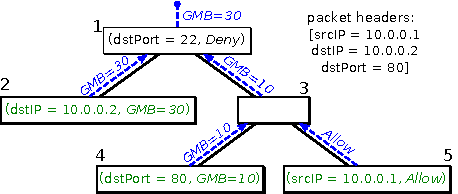
\includegraphics{figs/evaltree}
\caption{Evaluation of a single packet}
\label{f:evaltree}
\end{figure}


\vspace{0.5em}\noindent\textbf{Example:\space}
Figure~\ref{f:evaltree} depicts a simple Policy Tree
and illustrates how $\mathit{eval}$ produces an action, given the 
tree and indicated packet.
Each node contains its policy atoms, and atoms which match the packet are colored
green. The $\mathit{eval}$ function recursively produces an action from
each sub-tree; these actions are the labels on each node's outgoing edge.

In this example, the policy atoms at each leaf match the packet and produce
an action.
Node $3$ receives conflicting actions
from its children, which it resolves with its inter-sibling
conflict-resolution operator:
$\textbf{GMB}(10)
+_S \textbf{Allow} = \textbf{GMB}(10)$. Node $3$ has no policy atoms
itself, so it produces the $\textbf{0}$ action. Since $\textbf{0}$ is
the identity of all conflict-resolution operators,
  $\textbf{0} +_P \textbf{GMB}(10) = \textbf{GMB}(10)$ is the
resulting action from this sub-tree. 

Finally, Node 1 computes the aggregate action of its children:
$\textbf{GMB}(30) +_S \textbf{GMB}(10) = \textbf{GMB}(\max(30,10))$.
Since Node 1's policy atoms do not match the packet,
the final action is
$\textbf{0} +_P \textbf{GMB}(30) = \textbf{GMB}(30)$.

%%%%%%

\section{Compilation {\color{red} (Linearization?)}}
\label{sec:compilation}

The preceding chapter assumes that a central function,
$\mathit{eval}$, observes and directs all packets in the network.
Although $\mathit{eval}$ specifies the meaning of Policy Trees, this is not a
practical implementation. We now describe how to compile {\color{red}(flatten?)}
Policy Trees to run on commodity OpenFlow switches, which support simpler, linear
flow tables, to produce a practical implementation.

This process proceeds in two stages. First, we translate Policy Trees to
\emph{network flow tables}, which have a basic,
linear matching semantics. Second, \sys's runtime uses
network flow tables to configure a distributed network of switches,
translating high-level actions such as $\textbf{GMB}(n)$ to low-level
operations on switches. We defer discussion of \sys's runtime until
\Cref{sec:FullSystem}.

\begin{figure}[t]

\begin{displaymath}
\begin{array}{lrcl}
\textrm{Network Flow Tables} & N & = & \langle \overrightarrow{M,A} \rangle
\end{array}
\end{displaymath}

\fbox{$\mathit{scan} : N \times K \rightarrow A$}

\medskip

\inference
{M_1\cap K = \emptyset \cdots M_{j-1} \cap K = \emptyset \qquad
 M_j\cap K \ne \emptyset }
{\mathit{scan}(\langle(M_1,A_1)\cdots(M_n,A_n)\rangle,K) = A_j}

\medskip

\inference
{M_1\cap K = \emptyset \cdots M_{n} \cap K = \emptyset}
{\mathit{scan}(\langle(M_1,A_1)\cdots(M_n,A_n)\rangle,K) = \textbf{0}}

\medskip

\fbox{$\mathit{lin}_D : D \rightarrow N$}
\begin{displaymath}
\begin{array}{l}
\mathit{lin}_D\left(+_D,\{M_1,A_1, \cdots, M_j,A_j \}\right) 
  = N_1 \\
\begin{array}{lllll}
\textrm{where} 
& N_1 = \mathit{union}(+_D,\langle M_1,A_1\rangle, N_2) \\
& \cdots \\
& N_j = \mathit{union}(+_D, \langle M_j,A_j\rangle, \langle\rangle)
\end{array}
\end{array}
\end{displaymath}

\fbox{$\mathit{lin}_T : T \rightarrow N$}
\begin{displaymath}
\begin{array}{l}
\mathit{lin}_T\left(+_P,+_S,D, \{T_1\cdots T_k\}\right)
  = \mathit{union}(+_P,\mathit{lin}_D(D), N_1) \\
\begin{array}{lllll}
\textrm{where} 
& N_1 = \mathit{union}(+_S, \mathit{lin}_T(T_1), N'_2) \\
& \cdots \\
& N_k = \mathit{union}(+_S,\mathit{lin}_T(T_k), \langle \rangle)
\end{array}
\end{array}
\end{displaymath}

\fbox{$\mathit{union},\mathit{inter} : (+) \times N \times N \rightarrow N$}
\begin{displaymath}
\begin{array}{l}
\mathit{union}((+),N_1,N_2) = \mathit{inter}((+),N_1,N_2) N_1 N_2 \\
\mathit{inter}((+),\langle\cdots(M_i,A_i)\cdots\rangle, \langle\cdots(M'_j,A'_j)\cdots\rangle) = \\
\qquad \langle\cdots(M_i \cap M'_j,A_i+A'_j))\cdots\rangle
\end{array}
\end{displaymath}

\caption{Network Flow Tables}
\label{f:intermediate}

\end{figure}

A network flow table ($N$) is a sequence of paired match rules
and actions. The $\mathit{scan}$ function, defined in
Figure~\ref{f:intermediate}, matches packets against network flow
tables and returns the action associated with the first matching rule. If
no rules match the packet, then $\mathit{scan}$ returns $\textbf{0}$.\footnote{The
  $\mathit{scan}$ function is derived from 
  NetCore~\cite{Monsanto:2012} and presented as a \emph{type judgement}
  in the figure.}

The matching semantics of network flow tables correspond to the
matching semantics of switch flow tables exposed by OpenFlow.  When a
packet matches a switch flow table, only one rule's action applies. If a
packet matches multiple rules, the switch selects the one with the
highest priority.  A rule's index in a network flow table corresponds
to a switch flow table priority, with index $0$ as the highest
priority. Since all rules have distinct indices, a naive
correspondence would give all rules distinct priorities. A more
compact one, which we use, maps a sequence of
non-overlapping network flow table rules to a single priority in a
switch flow table.

The $\mathit{lin}_T$ function is our compiler from Policy Trees to
network flow tables. It uses $\mathit{lin}_D$ as a helper to compile
Policy Tree nodes.  The $\mathit{lin}_D$ function translates policy
atoms to singleton network flow tables, and combines them with
$\mathit{union(+,N_1,N_2)}$.  $\mathit{Union}$ builds a network flow table that
matches packets in either $N_1$ or $N_2$. In particular, when a packet
matches both $N_1$ and $N_2$, $\mathit{union}$ computes the intersection
using the $+$ conflict-resolution operator to combine
actions; in Figure~\ref{f:intermediate} we write the definition of
$\mathit{union}$ as the table produced by $\mathit{inter(+,N_1,N_2)}$ prepended
to the concatenation of $N_1$ and $N_2$.

Similarly, $\mathit{lin}_T$ recursively builds network flow tables for
its subtrees, and calls $\mathit{lin}_D$ on its root node.  It applies
$\mathit{union}$ to combine the results, using $+_S$ and $+_P$ where
appropriate.


The functions in Figure~\ref{f:intermediate}, $\mathit{lin}_T$,
$\mathit{lin}_D$, $\mathit{union}$, and $\mathit{inter}$ require the
conflict-resolution operators to satisfy the following properties.
\begin{wftree}[Well-formed] 
$T$ is well-formed if:
\begin{itemize}

\item All conflict-resolution operators are associative, and

\item $\textbf{0}$ is the identity of all conflict-resolution operators.
\end{itemize}
\end{wftree}
Proving the compiler correct requires the following key lemma, which
states that all conflict-resolution operators distribute over $\mathit{scan}$.
\begin{unioncommute}
For all $+$, $N_1$, and $N_2$, where $\textbf{0}$ is the identity of $+$,
$\mathit{scan}(\mathit{union}(+,N_1,N_2)) = \mathit{scan}(N_1) +
\mathit{scan}(N_2)$.
\end{unioncommute}
With this, we prove the compiler correct.
\begin{compilercorrect}[Soundness]
For all well-formed Policy Trees, $T$ and packets, $P$, $\mathit{eval}(T, P) =
\mathit{scan}(\mathit{lin}_T(T), P)$.
\end{compilercorrect}
We mechanize all our definitions and proofs using the Coq proof assistant~\cite{coq}. \qed

\section{Discussion}

{\color{red}
HotSDN reviewer
2 wanted to understand how \sys's use of the tree was an improvement over FML (e.g.,
why we couldn't just compile to FML, in theory).
}

From the beginning, we have modeled \sys's dynamic semantics as a tree.
There is not, however, a fundamental reason why this tree couldn't have been a DAG.
\sys offers network administrators a way to decompose their authority into
individual capabilities for non-administrative principals. We find trees to simply
be a natural way to reason about and understand such hierarchical decomposition.

Generalizing \sys's semantics to use a DAG would introduce a number of difficulties
which our current design avoids. For example, a tree provides only a single path
to the root, which eliminates any potential for ambiguity when accounting for
resource consumption in the hierarchy. Furthermore, \sys's current design implies
that each share completely restricts any requests in its sub-shares; they cannot be
expanded by merging with other paths in a DAG. This helps administrators know
how much authority has been granted to users, which may assist physical planning
(\eg, for bandwidth-type restrictions).

To achieve some of the benefits of a more general approach, we could implement
``aggregate'' requests which draw from multiple shares. Such future work
would need to tackle problems with resource fragmentation, fairness, and work-conservation.
For example, \sys's current, simple approach prevents hoarding because users cannot
use resources from multiple shares to gather more than what any single path through
the tree has granted them.

\section{Complexity of Compilation}

{\color{red} AG: I believe this should go in the compiler chapter.}

The policy tree compilation algorithm in Figure~\ref{f:intermediate} requires
a small optimization to be practical.

First, consider the complexity of the unoptimized compilation
algorithm.  The compiler calculates the union of all policy atoms,
using the $\mathit{union}$ function.  The $\mathit{union}$ function
calls $\mathit{inter}$, which computes the cross product of two
network flow tables, $N_1$ and $N_2$. This cross product calculation
is an $O(|N_1|\cdot|N_2|)$ that produces a network flow table of size
$O(|N_1|\cdot|N_2|)$. The cross product has to be calculated at all
nodes of the policy tree. Therefore, in a tree of depth $d$, if the
network flow tables at the leaves have size $n$, the running time of
the compiler takes $O(n^{2^d})$ steps.

Fortunately, a simple optimization makes the compiler tractable. We compact
all network flow tables as follows:
\begin{itemize}

\item We remove all entries with empty patterns, and

\item We remove entries whose patterns are fully shadowed by higher-priority
  entries.

\end{itemize}

\section{Conflict-resolution Operators}
\label{sec:conflict-resolution-operators}

\begin{figure}[t]

\fbox{$+_P : A \times A \rightarrow A$}
\begin{displaymath}
\begin{array}{lclcl}
A_P & +_P & \textbf{0} & = & A_P \\
\textbf{0} & +_P & A_C & = & A_C \\
\textbf{Deny} & +_P & \textbf{Allow} & = & \textbf{Allow} \\
\textbf{Allow} & +_P & \textbf{Allow} & = & \textbf{Allow} \\
A_P & +_P & \textbf{Deny} & = & \textbf{Deny} \\
\textbf{Deny} & +_P & \textbf{GMB}(n) & = & \textbf{GMB}(n) \\
\textbf{GMB}(m) & +_P & \textbf{GMB}(n) & = & \textbf{GMB}(\max(m,n)) \\
\textbf{GMB}(m) & +_P & \textbf{Allow} & = & \textbf{GMB}(m) \\
\textbf{Allow} & +_P & \textbf{GMB}(m) & = & \textbf{GMB}(n)
\end{array}
\end{displaymath}

\fbox{$+_S,+_D : A \times A \rightarrow A$}
\begin{displaymath}
\begin{array}{lclcl}
A_1 & +_S & \textbf{0} & = & A_1 \\
\textbf{0} & +_S & A_2 & = & A_2 \\
\textbf{Deny} & +_S & A_2 & = & \textbf{Deny} \\
A_1 & +_S & \textbf{Deny} & = & \textbf{Deny} \\
\textbf{GMB}(m) & +_S & \textbf{GMB}(n) & = & \textbf{GMB}(\max(m,n)) \\
\textbf{GMB}(m) & +_S & \textbf{Allow} & = & \textbf{GMB}(m) \\
\textbf{Allow} & +_S & \textbf{GMB}(m) & = & \textbf{GMB}(m) \\
\textbf{Allow} & +_S & \textbf{Allow} & = & \textbf{Allow} \\
A_1 & +_D & A_2 & = & A_1 +_S A_2 
\end{array}
\end{displaymath}

\caption{\sys's conflict-resolution operators}
\label{f:sysconflicts}

\end{figure}

Conflicts arise naturally in a participatory network, as \sys is
designed to allow multiple, distributed principals to author each Policy Tree.
For example, one principal may issue a request to deny traffic to
TCP port 80, while another may request  such traffic be allowed. \sys's
conflict-resolution operators determine the eventual outcome. These
operators take two conflicting requests as input, and return a single
resolved request.

Policy Trees have different types of conflict-resolution operators at several
points in the tree (\ie, $+_D$, $+_P$, $+_S$ in Figure~\ref{f:sharesem}). 
These multiple types allow \sys to resolve different types of conflicts using
independent logic: $+_D$ is used to resolve conflicts between requests
using the same share, $+_P$ between conflicting requests in parent and
child shares, and $+_S$ to resolve conflicts between sibling shares.
This allows conflict resolution to make use of the hierarchy, making it
simple to express intuitive conflict resolutions such as ``child overrides
parent.''
Therefore, the choice of conflict-resolution operators is a key policy decision.

As we discuss in \Cref{sec:compilation}, \sys's design allows for complex
conflict-resolution operators, and could support different operators at
each node in the Policy Tree. However, our current implementation does
not support this degree of complexity; we chose simple operators in the
interest of user and administrator understanding.
Figure~\ref{f:sysconflicts} specifies \sys's conflict-resolution
operators. {\color{red}(What about other resources??)}
The parent-child operator ($+_P$) specifies a ``child
overrides parent'' policy for admission control. The $+_S$ and $+_D$
operators are identical, and specify a ``\textbf{Deny} overrides
\textbf{Allow} policy'' between siblings.

These operators' simple design is heavily influenced by \sys's
first come-first serve approach to granting requests -- for example,
the operators do not consider the principal who made the request;
each request is treated equally within its hierarchical context.
However, by taking advantage of this design flexibility, operators
which resolve conflicts by using priorities could be introduced.
Because such an approach would lead to previously accepted requests
being preempted, the \sys controller would need to maintain a
connection to each principal to provide preemption notifications.
Avoiding this complexity is an additional benefit of \sys's current,
simple approach.


%%%%%%

